% ==============================================================================
% LAB 117
% SIMULERING PÅ ELEKTRISKA KRETSAR
% --------------------------------
% Last updated <2015-02-22>
%
% Author:
% Jonas Sjöberg     <tel12jsg@student.hig.se>
% Oscar Wallberg    <tco13owg@student.hig.se>
%
% License:
% Creative Commons Attribution-NonCommercial-ShareAlike 4.0 International
% See LICENSE.md for full licensing information.
% ==============================================================================

% ==============================================================================
% INCLUDES AND CONFIGURATION
% ==============================================================================
\documentclass[11pt,a4paper]{article}
\usepackage[utf8]{inputenc}
\usepackage[swedish]{babel} % För svensk innehållsförteckning
\usepackage{siunitx} % (För dokumentation, kör i terminalen; texdoc siunitx)
\usepackage{amssymb}
\usepackage{amsmath}
\usepackage{amsfonts}
\usepackage{graphicx}
\usepackage{booktabs}
\usepackage{longtable} % Tables span across pages
\usepackage{microtype}
\usepackage{gensymb}
%\usepackage{tabto}
\usepackage{units}

\setlength\parindent{0pt} % Removes all indentation from paragraphs

% ==============================================================================
% DOCUMENT METADATA
% ==============================================================================
\title{EE466 \\ Lab 117 \\ Simulering på elektriska kretsar}

\author{\\
  Jonas Sjöberg\\
  Högskolan i Gävle,\\
  Elektronikingenjörsprogrammet,\\
  \texttt{tel12jsg@student.hig.se}\\
  \\
  Oscar Wallberg\\
  Högskolan i Gävle,\\
  Dataingenjörsprogrammet,\\
  \texttt{tco13owg@student.hig.se}\\}

\date{}
% ==============================================================================
\begin{document}
% ==============================================================================
\maketitle

\begin{center}
    \begin{tabular}{l r}
        Lab utförd: & ? Februari 2015 \\
        Instruktör: & Efrain Zenteno
    \end{tabular}
\end{center}

% ==============================================================================
% ABSTRACT
% ==============================================================================
\begin{abstract}
    Syftet med laborationen är att genom använda ett simuleringsverktyg pröva
    några av de grundläggande sambanden och satserna i likströmsläran, samt att
    förstå enkla växelströmskretsar. Dessutom bör studenten efter genomförd
    laboration få en förståelse för hur enklare kretsar kan simuleras.
\end{abstract}

\newpage

{
    %\hypersetup{linkcolor=black}
    \setcounter{tocdepth}{3}
    \tableofcontents
}

\newpage

% ==============================================================================
% SECTION: INTRODUKTION
% ==============================================================================
\section{Introduktion}\label{setup}
% ==============================================================================
% TODO: Allmän introduktion.


% ==============================================================================
% SECTION: 1 MÄTNING PÅ SERIESKRETS
% ==============================================================================
\section{Mätning på seriekrets}\label{}
% ==============================================================================
Seriekretsen enligt figur 1 kopplades upp i Multisim. 10 \si{\volt} valdes för spänningskällan.
\begin{figure}[htbp]
    \centering
        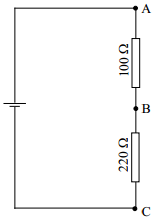
\includegraphics[scale=0.7]{misc/krets1.png}
    \caption{Seriekrets}
    \label{fig:1-mm-schem}
\end{figure}
\subsection{Mätresultat}\label{}
%För att mäta spänningarna vid punkt A, B samt C så placerades prober ut. Se figur 2 för resultat.
%TODO: Lägga in prntscrn/bild av koppling från multisim. ------------------------------------------------------------------------------
% TODO: Spänningarna mellan AB, BC och AC.

\subsection{Kommentar}\label{}
% ------------------------------------------------------------------------------
% TODO: Kommentera utgående från Kirchhoffs 2:a lag.
%       Kommentera utgående från spänningsdelningslagen.
Spänningsdelningslagen ger:\\
\begin{math}
U_{AB} = U\times\frac{R_{1}}{R_{1}+R_{2}}\\
U_{AB} = 10\times\frac{100}{100+220}\\
U_{AB} = 3.125\\
\\
U_{BC} = U\times\frac{R_{2}}{R_{1}+R_{2}}\\
U_{BC} = 10\times\frac{220}{100+220}\\
U_{BC} = 6.875\\
\\
\end{math}
Kirchhoff's 2:a lag:
\begin{quote}
Summan av samtliga emk:s som ingår i en sluten krets är lika med summan av potentialfallen, eller\\
\begin{math}
u_{1} + u_{2} + \ldots + u_{n} = 0\\
\text{där }u_{k} \text{ betecknar en potentialändring.}
\end{math}
\end{quote}
Enligt Kirchhoff's lag:\\
$U - U_{AB} - U_{BC} = 0$\\
$10 - 3.125 - 6.875 = 0$, vilket stämmer. %==============================================================================
% SECTION: 2 iNVERKAN AV EN PARALLELLGREN PÅ EN KRETS
% ==============================================================================
\section{Inverkan av en parallellgren på en krets}\label{}
% ==============================================================================
Ytterligare en resistor på 330 \si{\ohm} kopplades parallellt till kretsen från figur \ref{fig:1-mm-schem}, se figur \ref{fig:2-mm-schem}.
\begin{figure}[htbp]
    \centering
        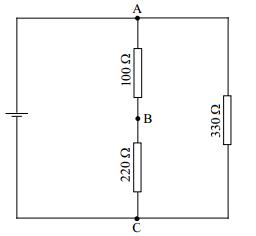
\includegraphics[scale=1.0]{misc/krets2.png}
    \caption{Parallellgren på föregående krets.}
    \label{fig:2-mm-schem}
\end{figure}
\subsection{Mätresultat}\label{}
% ------------------------------------------------------------------------------
% TODO: Mät strömmen i punkten B samt strömmen direkt från spänningskällan.


% ==============================================================================
% SECTION: 3 MÄTNING PÅ PARALLELLKRETS
% ==============================================================================
\section{Mätning på parallellkrets}\label{}
% ==============================================================================
Två resistorer kopplades enligt figur \ref{fig:3-mm-schem}. Sedan valdes en lämplig spänning för spänningskällan.
\begin{figure}[htbp]
    \centering
        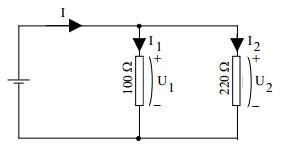
\includegraphics[scale=1.0]{misc/krets3.png}
    \caption{Parallellgren på föregående krets.}
    \label{fig:3-mm-schem}
\end{figure}

\subsection{Mätresultat}\label{}
% ------------------------------------------------------------------------------
% TODO: Mät de markerade strömmarna

\subsection{Kommentar}\label{}
% ------------------------------------------------------------------------------
% TODO: Kommentera utgående från Kirchhoffs 1:a lag.


% ==============================================================================
% SECTION: 4 MÄTNING AV RESISTANS
% ==============================================================================
\section{Mätning av resistans}\label{}
% ==============================================================================
Kretsarna funna i figur \ref{fig:4-mm-schem} kopplades.
\begin{figure}[htbp]
    \centering
        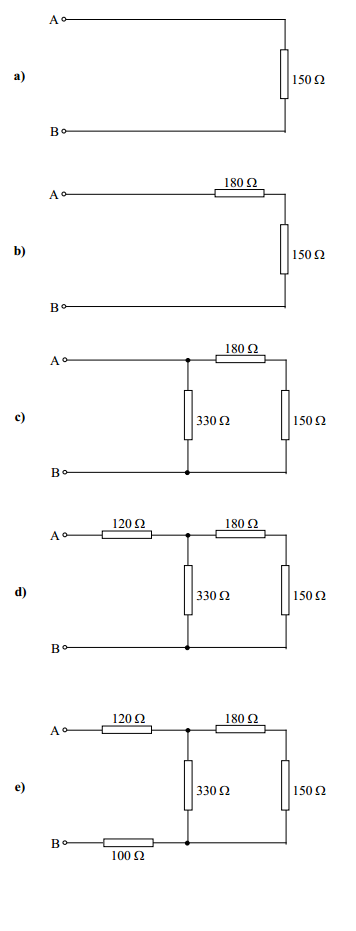
\includegraphics[scale=0.9]{misc/krets4.png}
    \caption{Resistorkretsar.}
    \label{fig:4-mm-schem}
\end{figure}
\subsection{Mätresultat}\label{}
% ------------------------------------------------------------------------------
% TODO: Mät resistansen mellan A och B i nedanstående kretsar.
a)\\
b)\\
c)\\
d)\\
e)

\subsection{Teoretisk beräkning}\label{}
% ------------------------------------------------------------------------------
% TODO: För varje mätning skall du verifiera resultatet med en teoretisk beräkning.


%\subsection{Kommentar}\label{}
% ------------------------------------------------------------------------------
% TODO: Kommentar på skillnader mellan mätresultat och beräkning?


% ==============================================================================
% SECTION: 5 STUDIUM AV FREKVENSGÅNG I EN REAKTIV KRETS
% ==============================================================================
\section{Studium av frekvensgång i en reaktiv krets}\label{}
% ==============================================================================
% TODO: Kopplingsschema.

\subsection{Mätresultat}\label{}
% ------------------------------------------------------------------------------
% TODO: + Gör upp en tabell som för varje frekvens anger
%         - tongeneratorns signalamplitud,
%         - amplituden hos spänningen över den studerade kondensatorn
%         - kvoten mellan den senare amplituden och den tidigare
%         - samt om fasförskjutning förekommer.

\subsection{Teoretisk beräkning}\label{}
% ------------------------------------------------------------------------------
% TODO: Kontrollera dina resultat genom att utnyttja följande formel:

\subsection{Kommentar}\label{}
% ------------------------------------------------------------------------------
% TODO:


% ==============================================================================
% SECTION: 6 MÄTNING AV FASFÖRSKJUTNING I EN REAKTIV KRETS
% ==============================================================================
\section{Mätning av fasförskjutning i en reaktiv krets}\label{}
% ==============================================================================
% TODO: Kopplingsschema.
%       Samma koppling som förra uppgiften, kanske överflödigt att upprepa?

\subsection{Mätresultat}\label{}
% ------------------------------------------------------------------------------
% TODO:

\subsection{Teoretisk beräkning}\label{}
% ------------------------------------------------------------------------------
% TODO: Kontrollera dina resultat genom att utnyttja följande formel:

\subsection{Kommentar}\label{}
% ------------------------------------------------------------------------------
% TODO: Kommentera resultatet


% ==============================================================================
% SECTION: 7 MÄTNING AV RESONANSFREKVENS
% ==============================================================================
\section{Mätning av resonansfrekvens}\label{}
% ==============================================================================
% TODO: Kopplingsschema.

\subsection{Mätresultat}\label{}
% ------------------------------------------------------------------------------
% TODO: Notera resonansfrekvensen.

\subsection{Kommentar}\label{}
% ------------------------------------------------------------------------------
% TODO: + Kommentera följande:
%         - Förekommer fasförskjutning mellan uTG och uR vid denna frekvens?
%         - Ändrar fasen sig om du varierar frekvensen kring den
%           uppmätta resonansfrekvensen?  I så fall hur?
%         - Om laboration 61 har gjorts, jämför resultatet med de uppmätta
%           värderna.  Stämmer de överens om inte, varför?


% ==============================================================================
% SECTION: RESULTAT
% ==============================================================================
\section{Resultat}\label{setup}
% ==============================================================================
% TODO: Övergripande resultat/sammanfattning/kommentar på HELA labben.

\newpage

% ==============================================================================
% SECTION: REFERENSER
% ==============================================================================
\section{Referenser}\label{refs}
% ==============================================================================
%TODO: Referenser.

%\subsection{www}\label{interwebs}
% ------------------------------------------------------------------------------

%\subsection{Trycksaker}\label{literature} %???
% ------------------------------------------------------------------------------

%\subsection{Källkod}\label{sourcefiles}
% ------------------------------------------------------------------------------

% ==============================================================================
\end{document}
% ==============================================================================
